\documentclass[12pt,a4paper,onecolumn]{article}
\usepackage{covington}
\usepackage{comment}
\usepackage{url}
\usepackage{mathtools}
\usepackage{tipa}
\usepackage[UKenglish]{babel}
\usepackage{graphicx}
\usepackage{subfigure}
\usepackage[font={it}]{caption}

% Spaced paragraphs
\setlength{\parindent}{0.0in}
\setlength{\parskip}{0.1in}


% Custom colors
\usepackage{color}
\definecolor{deepblue}{rgb}{0,0,0.5}
\definecolor{deepred}{rgb}{0.6,0,0}
\definecolor{deepgreen}{rgb}{0,0.5,0}

\usepackage{listings}
\lstset{
language=Matlab,
basicstyle=\ttfamily,
breaklines=true,
otherkeywords={self},             % Add keywords here
keywordstyle=\color{deepblue},
emph={MyClass,__init__},          % Custom highlighting
emphstyle=\color{deepred},    % Custom highlighting style
stringstyle=\color{deepgreen},
frame=tb,                         % Any extra options here
showstringspaces=false  
}

\newcommand{\code}[2]{
  \hrulefill
  \subsection*{#1}
  \lstinputlisting{#2}
  \vspace{2em}
}


\begin{document}
\title{AV Assignment 2: 3D Image Analysis}
\author{s0949775 and s1330128}
\date{\today}
\maketitle


\section{Introduction}
This report covers the construction of a 3D model from a 
sequence of RGB and depth frames from the Kinect. 
The algorithms we chose and explored are discussed for
each phase of processing:
\begin{itemize}
\item Extracting the bin from the RGB images and corresponding 3D points.
\item Aligning the extracted bin points from each frame in a single coordinate frame.
\item Combining the aligned bin points into a single dataset.
\item Fitting planes to the sides of the bin.
\end{itemize}

\section{Box Extraction}
To extract the bin we used a series of techniques on the colour and depth data.  We first converted the image to a chromaticity image, and smoothed with a gaussian filter to reduce noise.  This accentuated the orange regions of the box and made them consistent throughout the sequence.  An example image from this stage is shown in figure \ref{fig:full_chromaticity_image}.

We manually thresholded the smoothed chromaticity image, using separate thresholds for each of the three colour channels, to detect the orange regions.  The output from this stage is shown in figure \ref{fig:thresholding_result}.

\begin{figure}[h!]
    \centering
      \subfigure[RGB image converted to chromaticity coordinates and smoothed.]{
        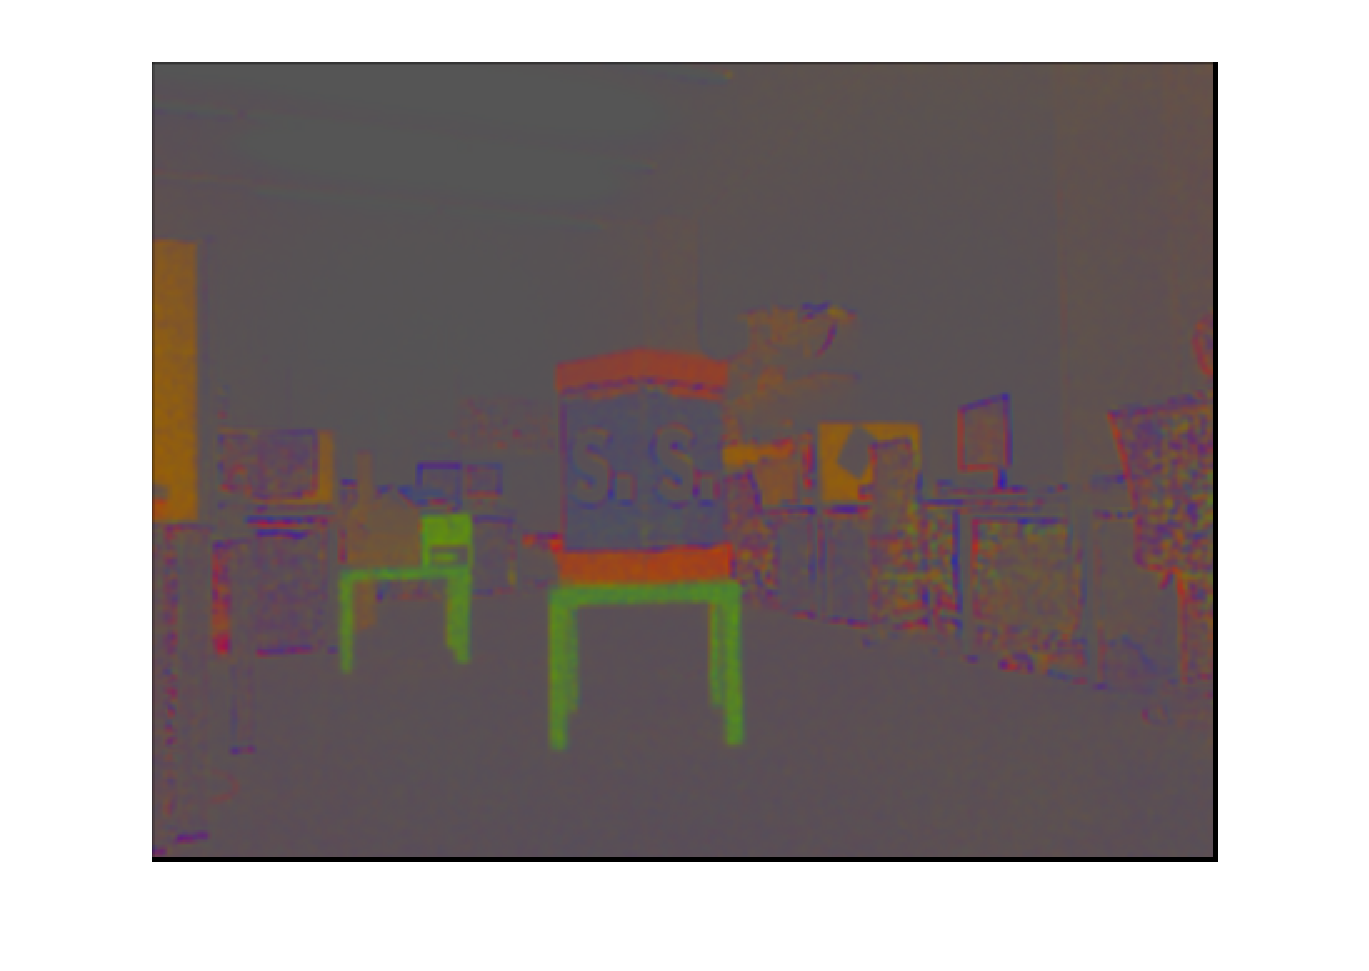
\includegraphics[width=0.45\linewidth]{figs/full_chromaticity_image}
        \label{fig:full_chromaticity_image}
      }
      \quad
      \subfigure[Thresholding colours to find orange regions.]{
        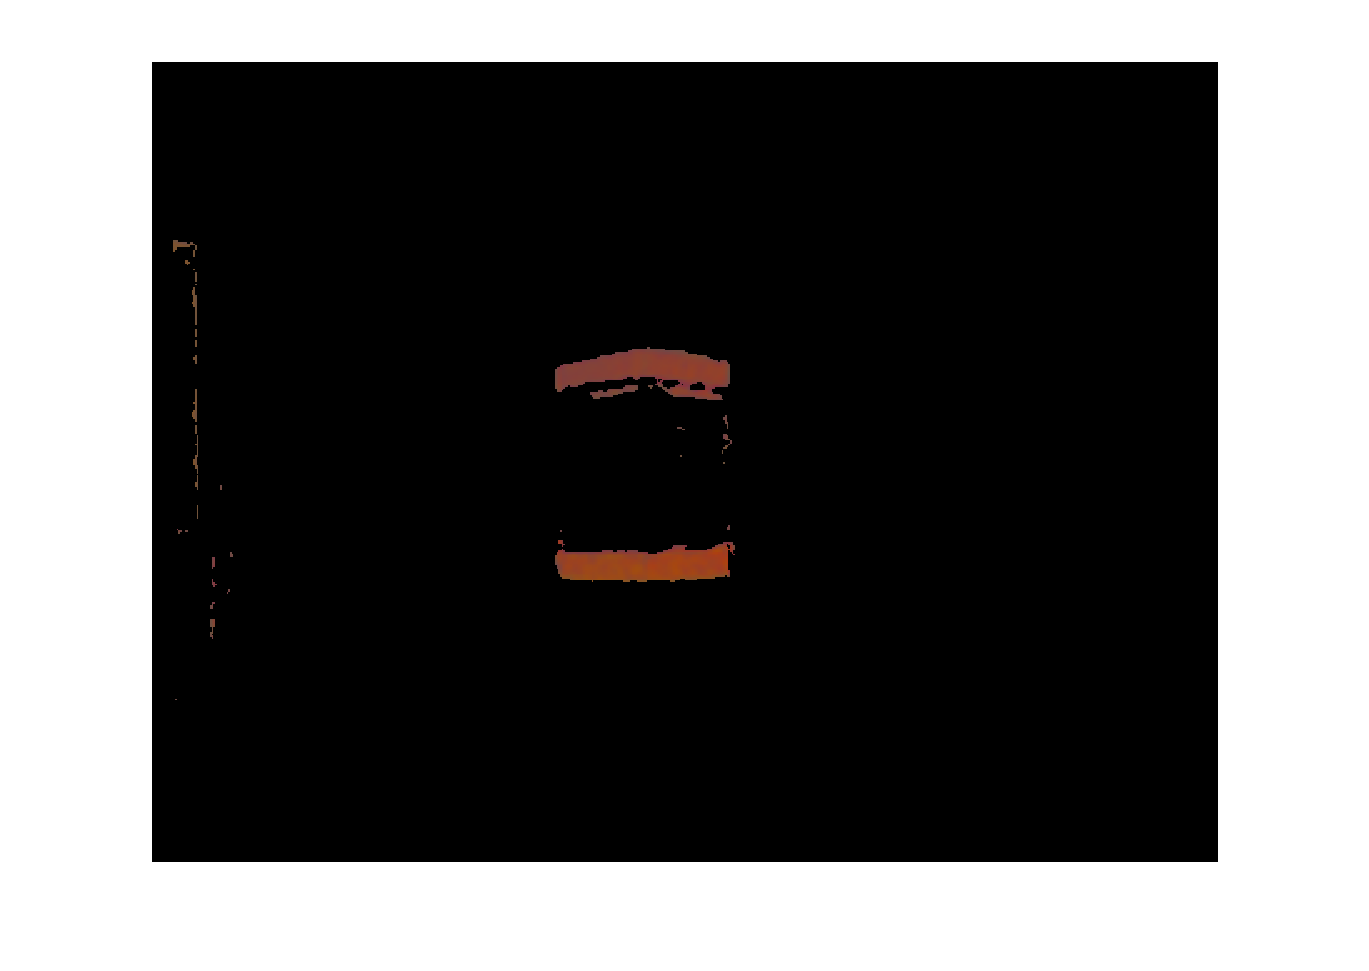
\includegraphics[width=0.45\linewidth]{figs/thresholding_result}
        \label{fig:thresholding_result}
      }

        \subfigure[Depth image.]{
        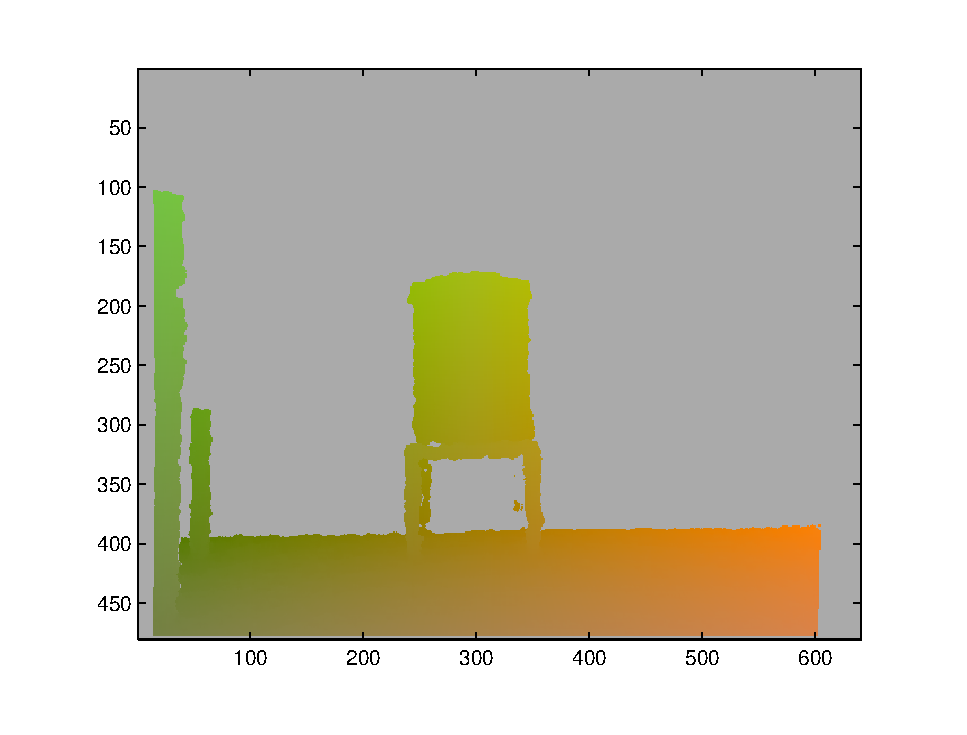
\includegraphics[width=0.45\linewidth]{figs/full_depth_data_picture}
        \label{fig:full_depth_data_picture}
      }
      \subfigure[Detected bottom of the bin.]{
        \includegraphics[width=0.45\linewidth]{figs/detected_bottom_orange_region_mask}
        \label{fig:detected_bottom_orange_region_mask}
      }
      \subfigure[Mask of detected bin]{
        
\includegraphics[width=0.45\linewidth]{figs/extracted_box_mask_example}
        \label{fig:extracted_box_mask_example}
      }
      \caption{Box extraction stages.}
\end{figure}

Some noise is present, which corresponds to other orange features in the scene.  To eliminate this, we took the intersection of the thresholded regions with the depth image (see figure \ref{fig:full_depth_data_picture}), and identified the two largest connected components remaining.  These corresponded to the orange regions at the top and bottom of the box.  From these we could reliably find the bottom of the box, as shown in figure \ref{fig:detected_bottom_orange_region_mask}.  Finally, to identify all of the pixels in the box, we took all pixels in the depth map that were above the bottom edge of the lower orange region (figure \ref{fig:extracted_box_mask_example}), to produce the colour image in figure \ref{fig:extracted_box_example}.

\begin{figure}[!ht]
  \centering
  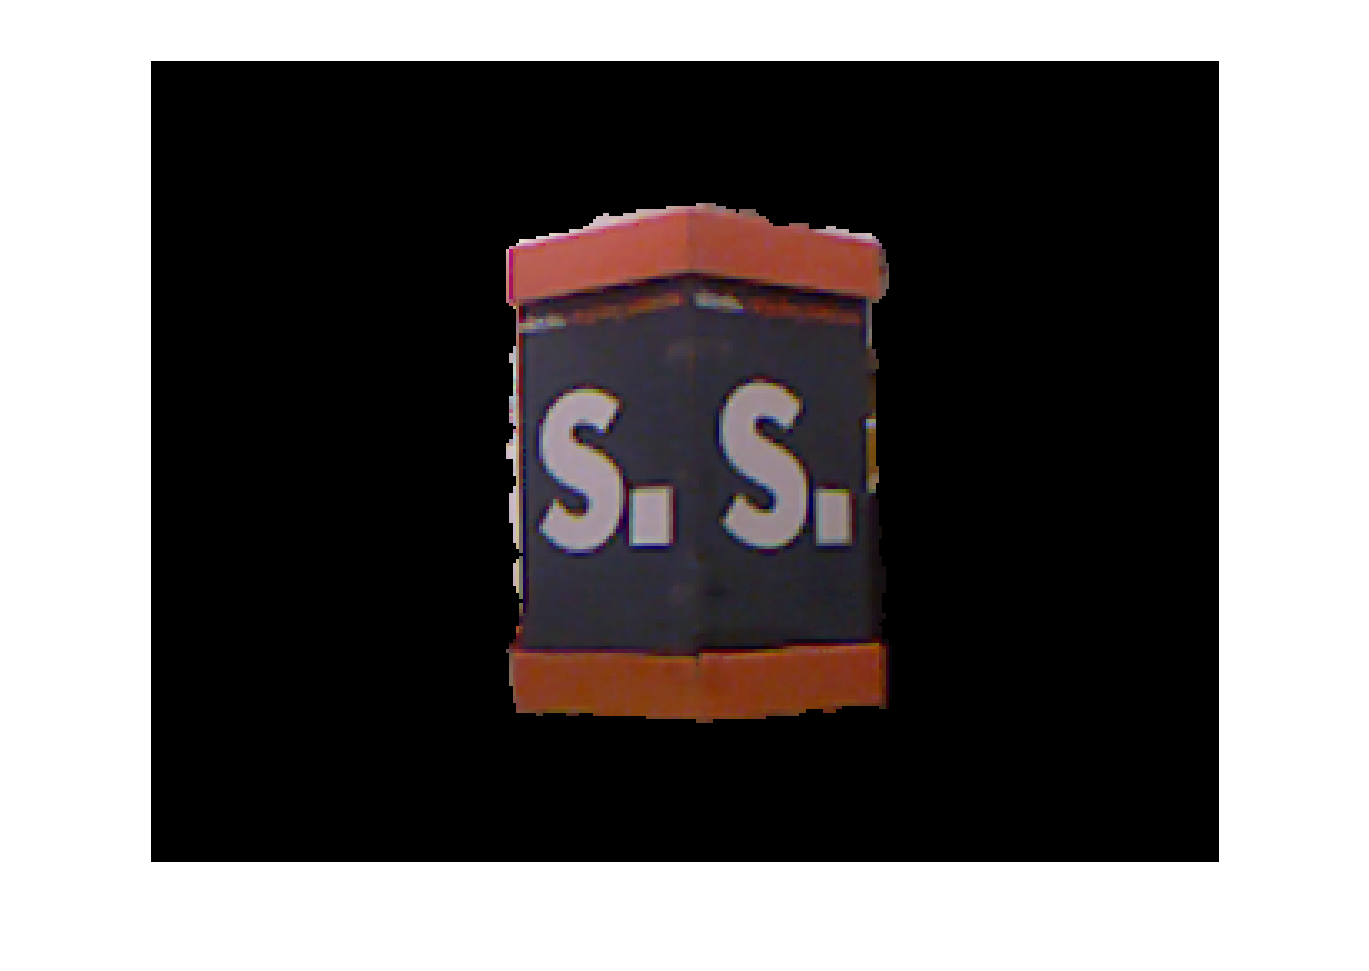
\includegraphics[width=1.0\textwidth]{figs/extracted_box_example}
  \caption{Final extracted box for one frame.}
  \label{fig:extracted_box_example}
\end{figure}

This technique worked well for the frames in the dataset, although it relied on knowledge specific to that dataset, such as the largest orange regions belonging to the box, and the box being isolated in the depth image.

The final image in figure \ref{fig:extracted_box_example} shows some noise around the box.  We tried removing this by using thresholds on the box pixels.  The noise could be removed quite effectively for individual frames, but no static threshold values worked over the whole sequence.  Adaptive thresholding could be used to deal with this, but we decided that the resulting box extraction was good enough for our purposes.

\begin{figure}[!h]
    \centering
      \subfigure[Depth point data from single frame.]{
        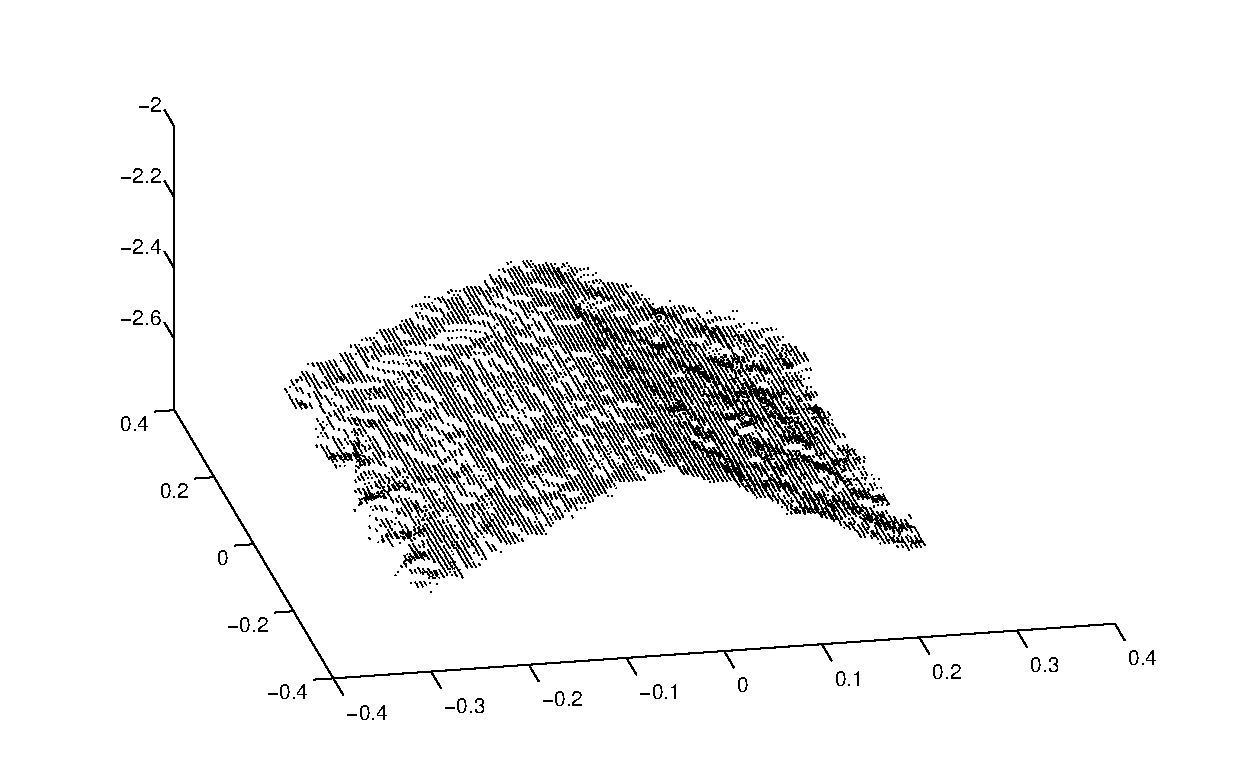
\includegraphics[width=0.475\linewidth]{figs/depth_points_example}
        \label{fig:depth_points_example}
      }
      \subfigure[Coloured depth points.]{
        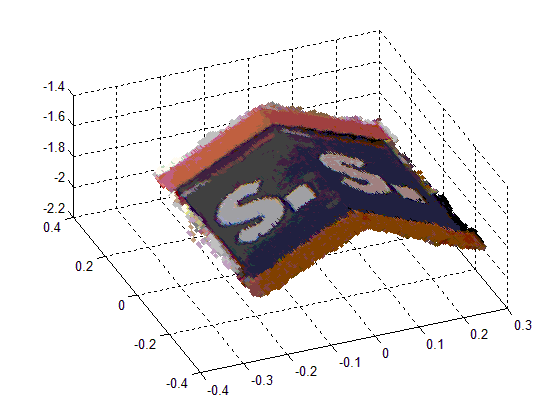
\includegraphics[width=0.475\linewidth]{figs/coloured_depth_points}
        \label{fig:coloured_depth_points}
      }
      \caption{3D Points of extracted bin.}
\end{figure}

\section{Point Alignment}
As was suggested in the assignment we took the middle frame
from the sequence as our foundation frame, against which we aligned all other frames.

To align points for different frames we used the ICP algorithm
linked to in the assignment.  Because the plane points are not very distinctive, we used the edge points for alignment.  We detected the edges using Canny edge detection on the extracted RGB box pixels, converted to greyscale.  We tuned the edge detector parameters to ensure that only the main edges of the box were detected, as in figure \ref{fig:extracted_edge_mask}.

\begin{figure}[h]
  \centering
  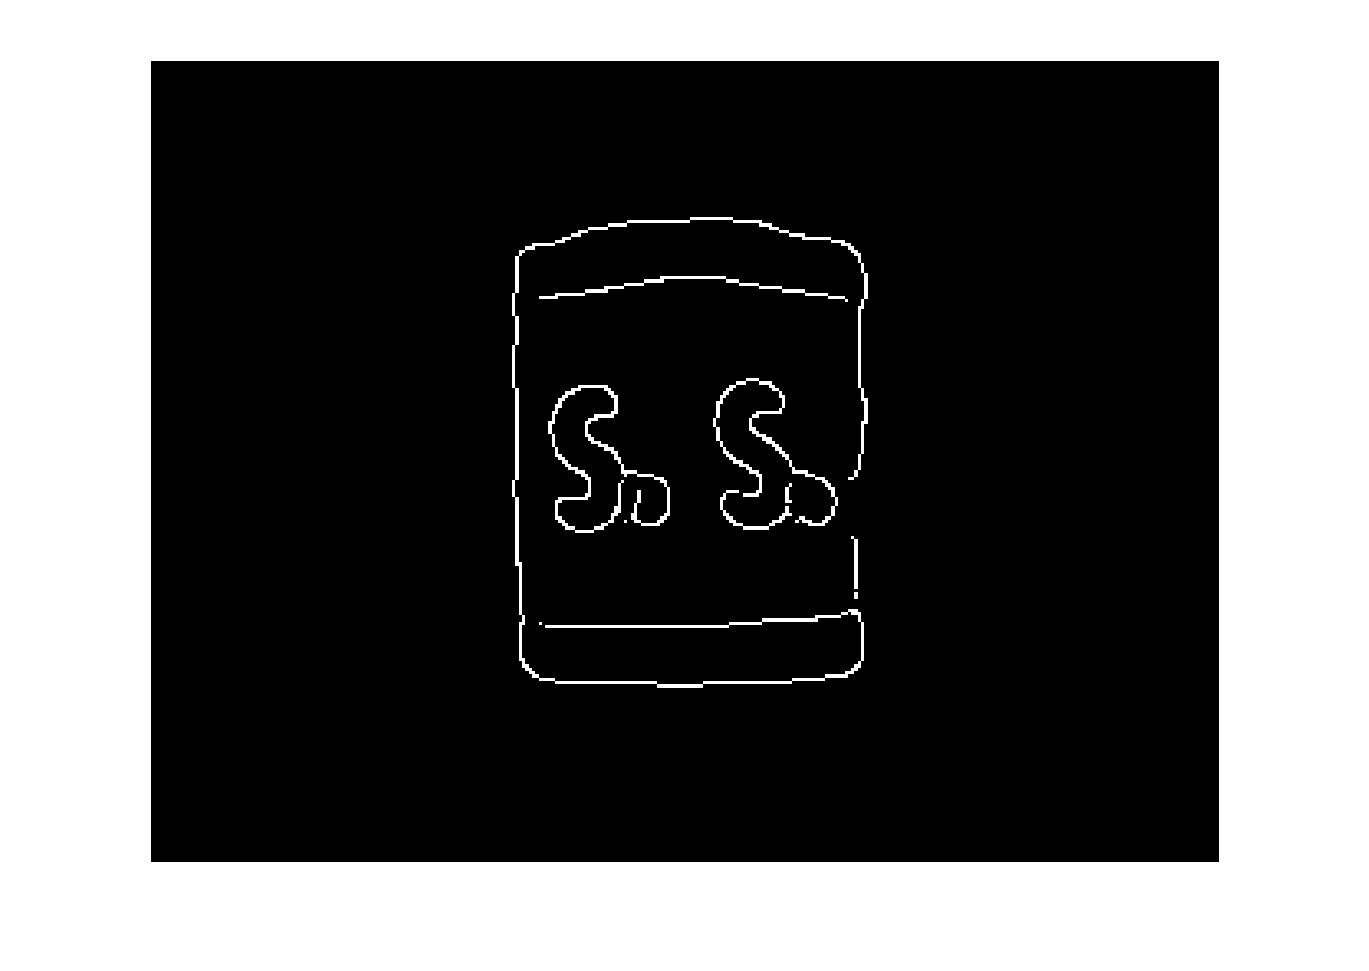
\includegraphics[width=0.5\textwidth]{figs/extracted_edge_mask}
  \caption{Extracted edges for ICP alignment}
  \label{fig:extracted_edge_mask}
\end{figure}

\begin{figure}[h]
    \centering
      \subfigure[ICP alignment with edge points - top view.]{
        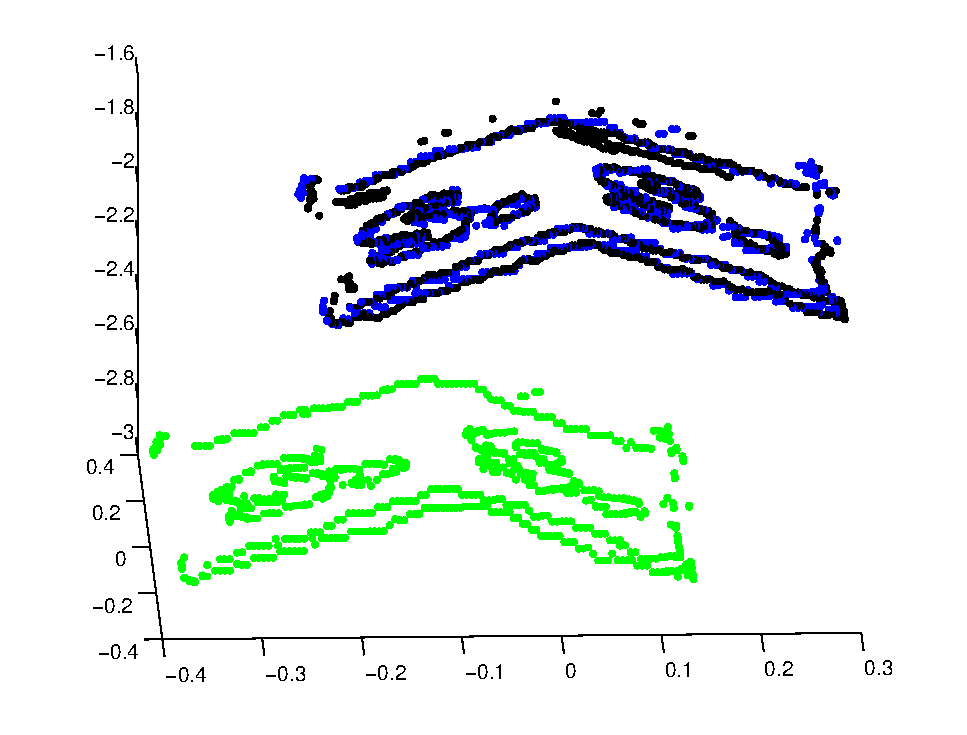
\includegraphics[width=0.475\linewidth]{figs/icp_before_alignment_from_side}
        \label{fig:icp_before_alignment_from_side}
      }
      \subfigure[ICP alignment with edge points - side view.]{
        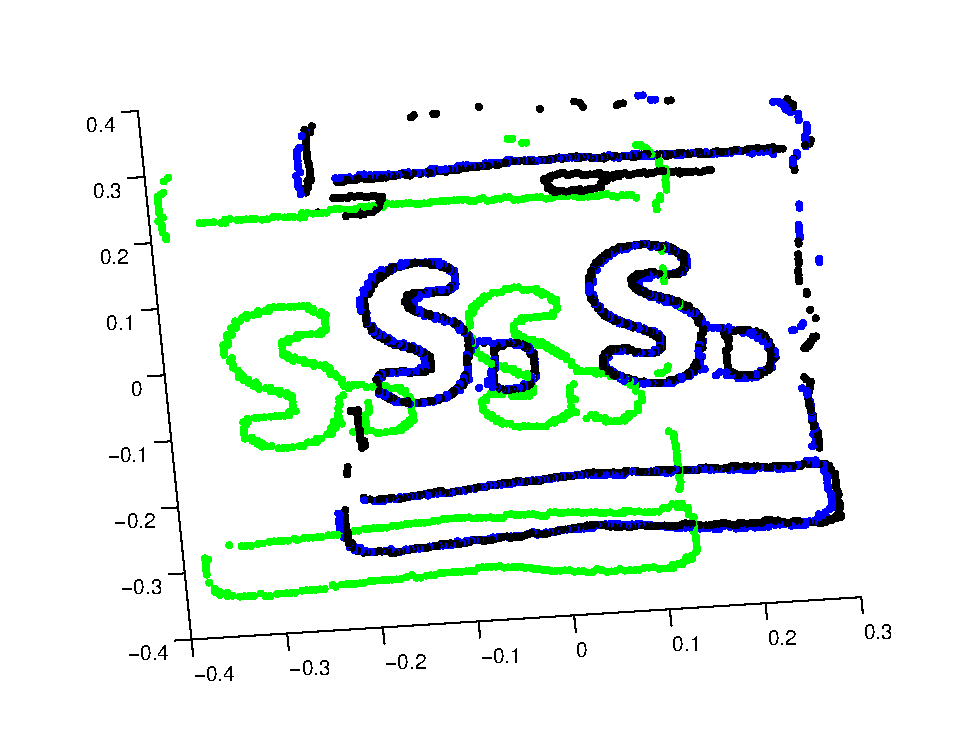
\includegraphics[width=0.475\linewidth]{figs/icp_before_alignment_from_top}
        \label{fig:icp_before_alignment_from_top}
      }
      \caption{ICP alignment.  The foundation frame is black.  The current frame is shown in green prior to alignment and blue after alignment.}
\end{figure}

We took the 3D points corresponding to the detected greyscale edges and used them as input to the ICP algorithm.  Figures \ref{fig:icp_before_alignment_from_side} and \ref{fig:icp_before_alignment_from_top} show an example alignment from the top and the side.

We found that aligning with the edges alone produced good results, and we did not see an improvement when using all the points in the bin.  Figure \ref{fig:depth_points_after_edge_point_icp_alignment_ok} shows the results of an alignment with just edge points, while figure \ref{fig:depth_points_after_full_point_icp_alignment_ok} shows the alignment using a combined transformation from edge points and all the points.  There was no clear visual difference.  Using the edges alone was also much faster than using all the points.

Fusing the data from each frame into a single composite dataset was a simple matter of concatenating the lists of points from all frames.

\begin{figure}[h]	
    \centering
      \subfigure[Depth point alignment using ICP transformations estimated only with edge points.]{
        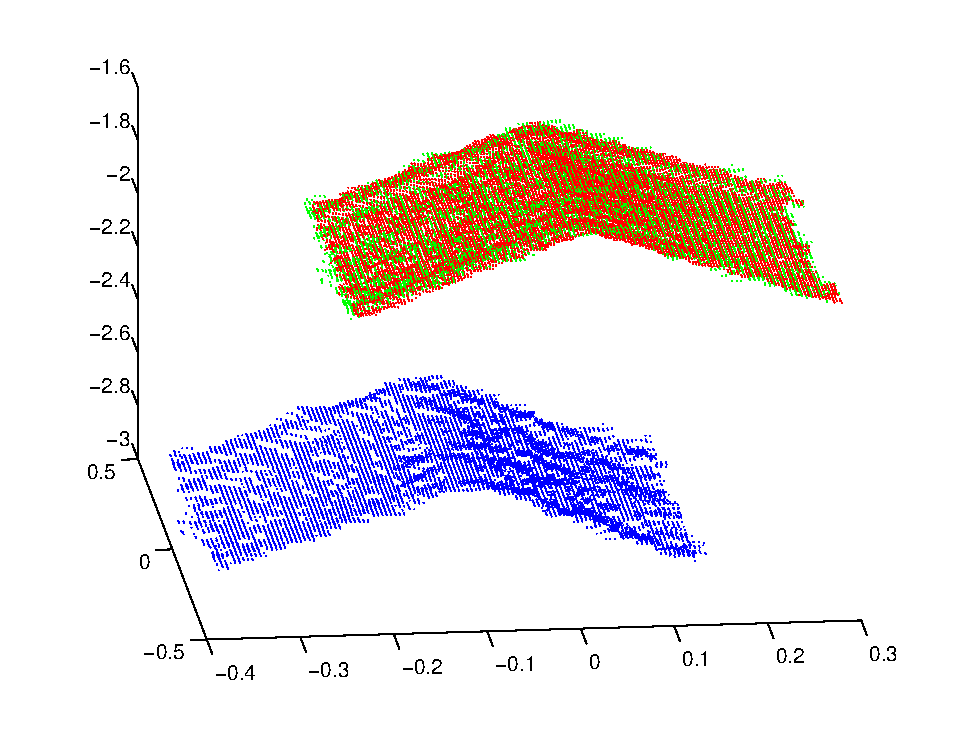
\includegraphics[width=0.475\linewidth]{figs/depth_points_after_edge_point_icp_alignment_ok}
        \label{fig:depth_points_after_edge_point_icp_alignment_ok}
      }
      \subfigure[Depth point alignment using ICP transformations estimated with 
      weighted edge points and full point set.]{
        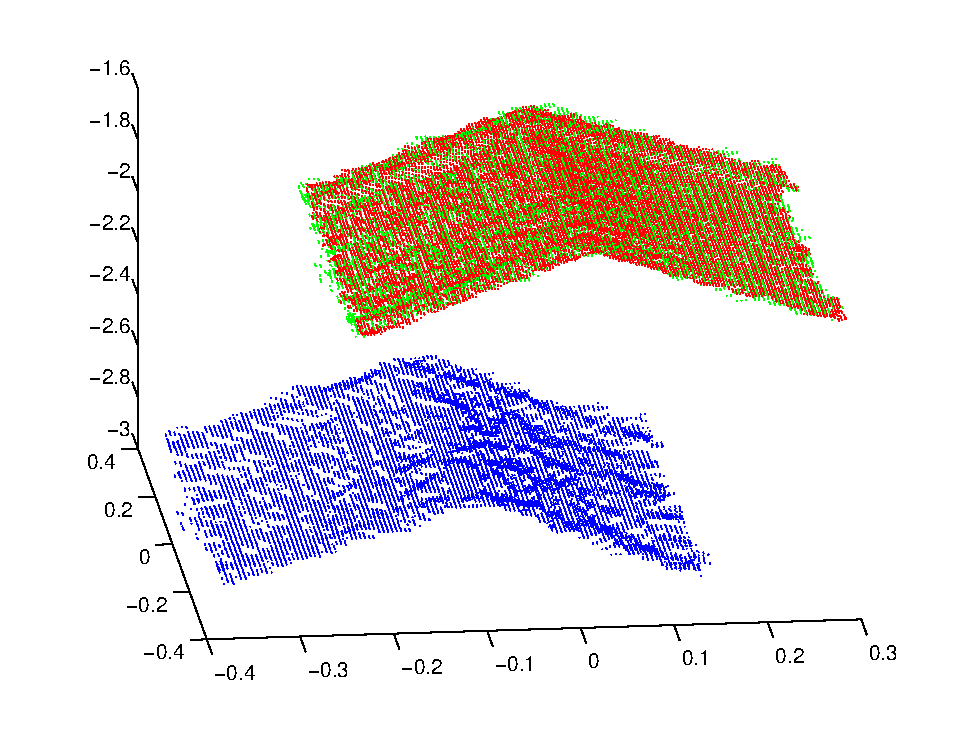
\includegraphics[width=0.475\linewidth]{figs/depth_points_after_full_point_icp_alignment_ok}
        \label{fig:depth_points_after_full_point_icp_alignment_ok}
      }
      \caption{Alignment of entire point dataset for the box. Red points are depth points from
      foundation frame, blue ones are from current frame for alignment and green ones (overlapping with red)
      are blue points after applying transformations estimated with ICP}
\end{figure}

\section{Plane Fitting}
For the plane fitting we implemented a modified K-means algorithm.  It starts with two randomly initialised planes and assigns points to the geometrically nearest plane.  The planes are then refitted to their points and all points are reassigned to the nearest plane.  This continues until the algorithm converges (the point assignments no longer change after the planes are refitted).  The code for this can be found in appendix \ref{apen:code_in}.

This approach easily allowed us to fit data points to any of number of
planes.  K-means is sensitive to the initialisation of the means.  A poor initialisation means that the algorithm will not converge to the correct answer.  To cope with this, we introduced thresholds
to find cases when initialisation was definitely wrong.  For example, if all the points were assigned to one plane we would reinitialise, and if the average plane fitting error was too high after convergence we would also reinitialise.  With these measures, the algorithm reliably and accurately fits two planes to the composite set of bin points from all frames.

We found that the angle between the planes was 60.2 degrees.  This was surprising as we expected it to be 90 degrees, and the planes appeared to be visually fitted well.

\begin{figure}[h]
    \centering
      \subfigure[Fitted planes]{
        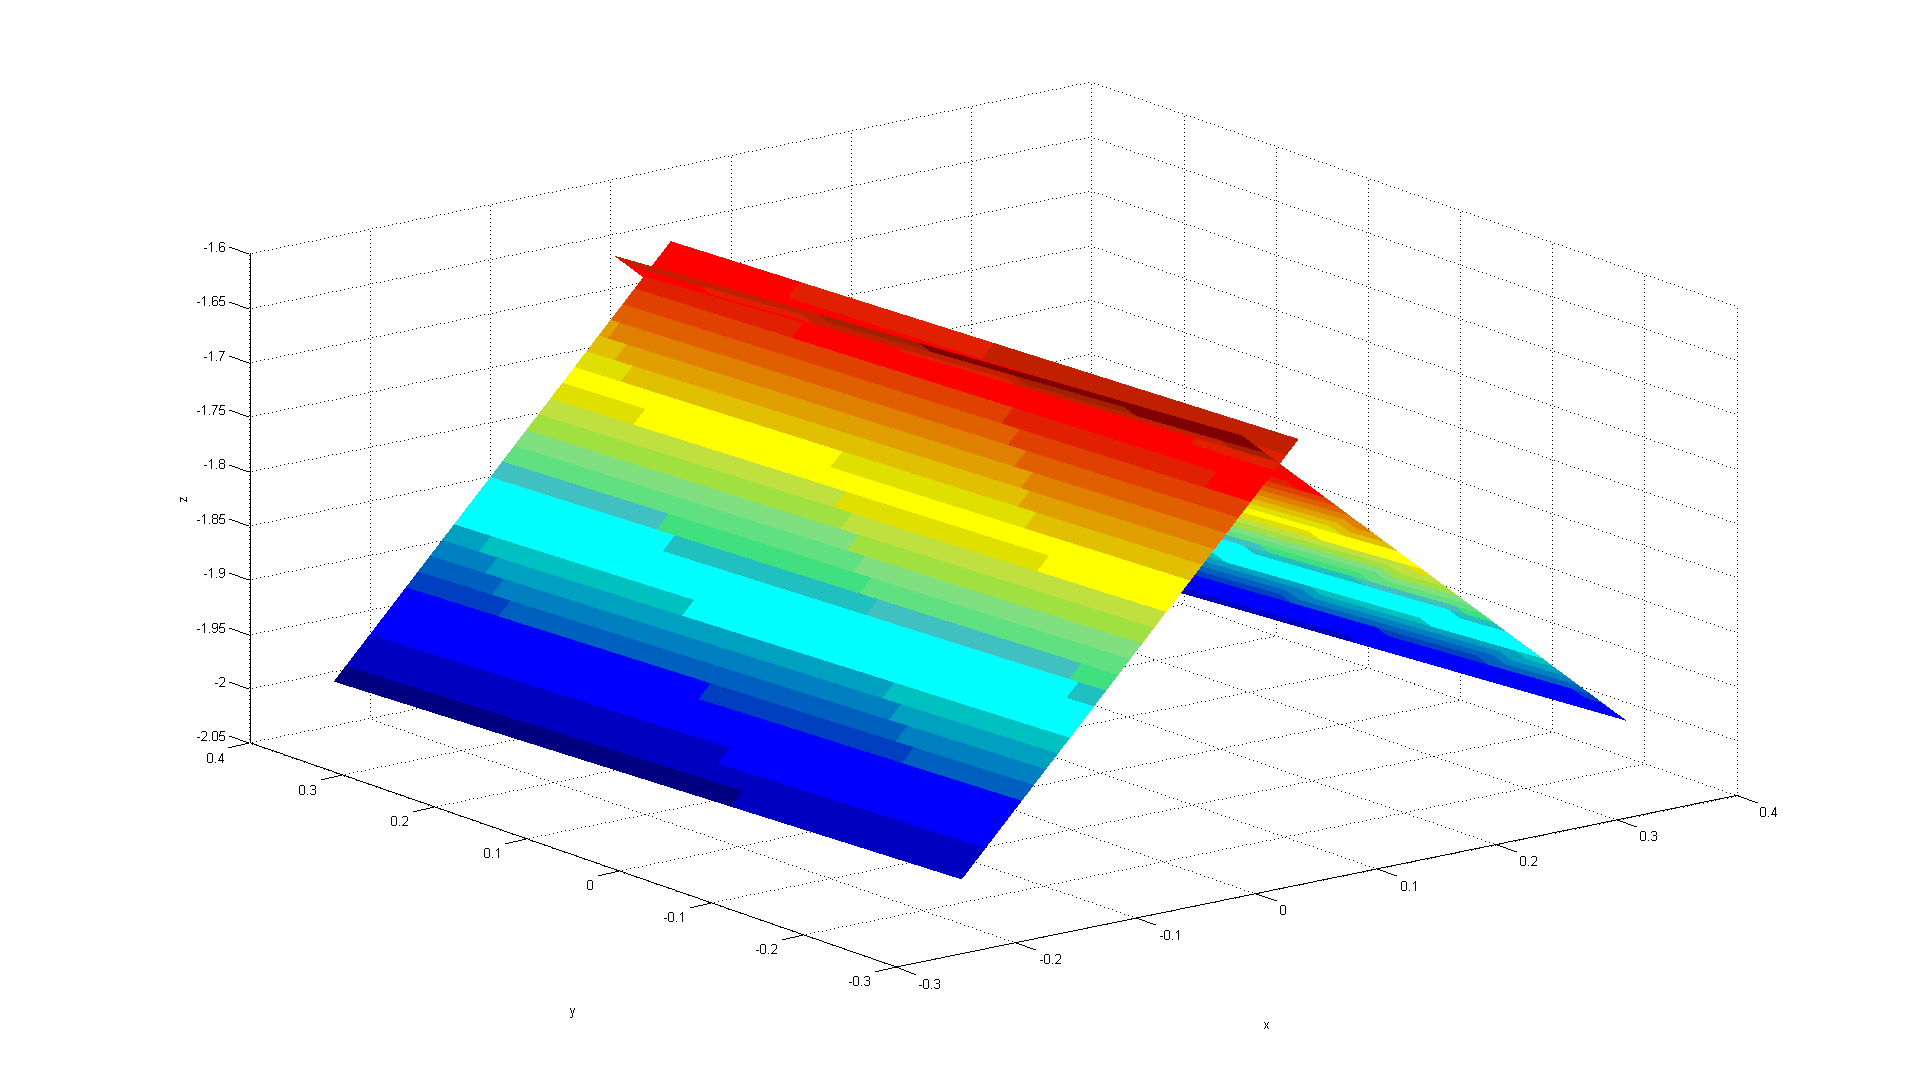
\includegraphics[width=0.475\linewidth]{figs/fitted_planes_without_points}
        \label{fig:fitted_planes_without_points}
      }
      \subfigure[Fitted planes together with final combined depth points]{
        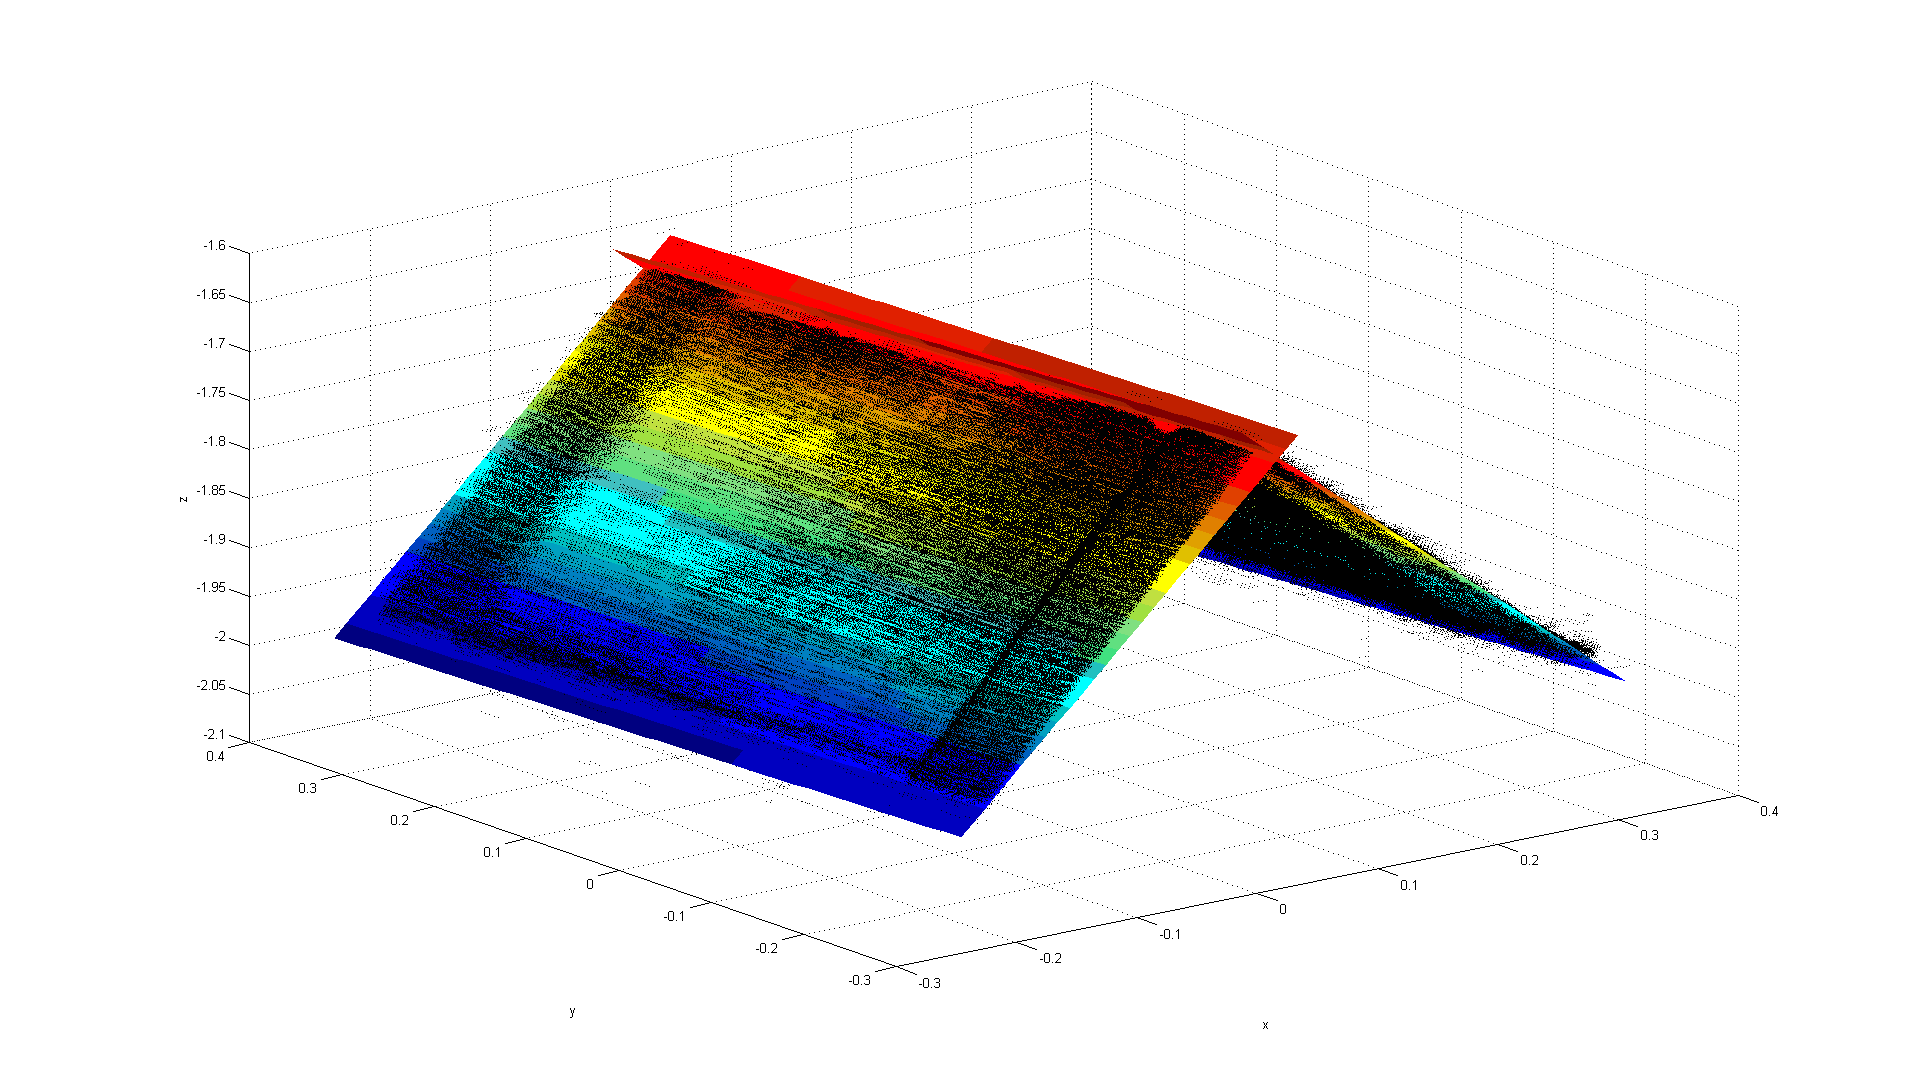
\includegraphics[width=0.475\linewidth]{figs/fitted_planes_with_points}
        \label{fig:fitted_planes_with_points}
      }
      \caption{Merged depth points shown together with fitted planes.}
\end{figure}

\section{Discussion}
The ICP and plane fitting algorithms worked without problems in most cases. K-means sometimes suffered
from poor initialisations but that was easily fixed using a few checks of total
absolute error. The trickiest part was initial box
region detection. Fine-tuning colour thresholds is a tedious
process and tends to capture some artefacts around the box
that might affect later stages.  In addition, finely tuned algorithms can work well for a specific dataset, but will probably not generalise as well.

One possible technique for box detection
would involve probabilistic background modelling - it might be possible
to detect the background from the whole series of frames
and then subtract it from each frame individually. 
We didn't try this, but stuck with the
simple approach that works well for our dataset.

\section{Evaluation}

Images of the bin after each dataset is merged can be seen in figures \ref{fig:eval1a} through \ref{fig:eval1b}, showing the composite points becoming more dense as each new frame is registered to the foundation frame.  They show the coloured and uncoloured 3D points from the top and the side.

Zoomed images of the leftmost white square as new frames are included are shown in figures \ref{fig:eval2a} and \ref{fig:eval2b}.

We extracted the surface normal of each of the rightward facing planes from the 20 images after the registration transformation and inverted if necessary to make sure that they all faced towards the camera.  We computed the angle between each vector and the Foundation vector, finding an average of 0.46 degrees with a standard deviation of 0.22.

Figure \ref{fig:plane_angle_error_versus_foundation_plane} shows the average distance of points in the rightmost S. region of the box to the local plane, as a function of the number of frames in the composite dataset.  It
can be seen that fitting error increases initially but starts to decrease
after the 10th frame. We think this may be because
 alignment is done against the foundation frame, and
the first frames are quite different from the foundation frame,
resulting in a higher error.  In addition, as more frames are included in the composite dataset, the effects of outliers will be reduced as most of the points will be concentrated near the plane.

\begin{figure}[h]
  \centering
  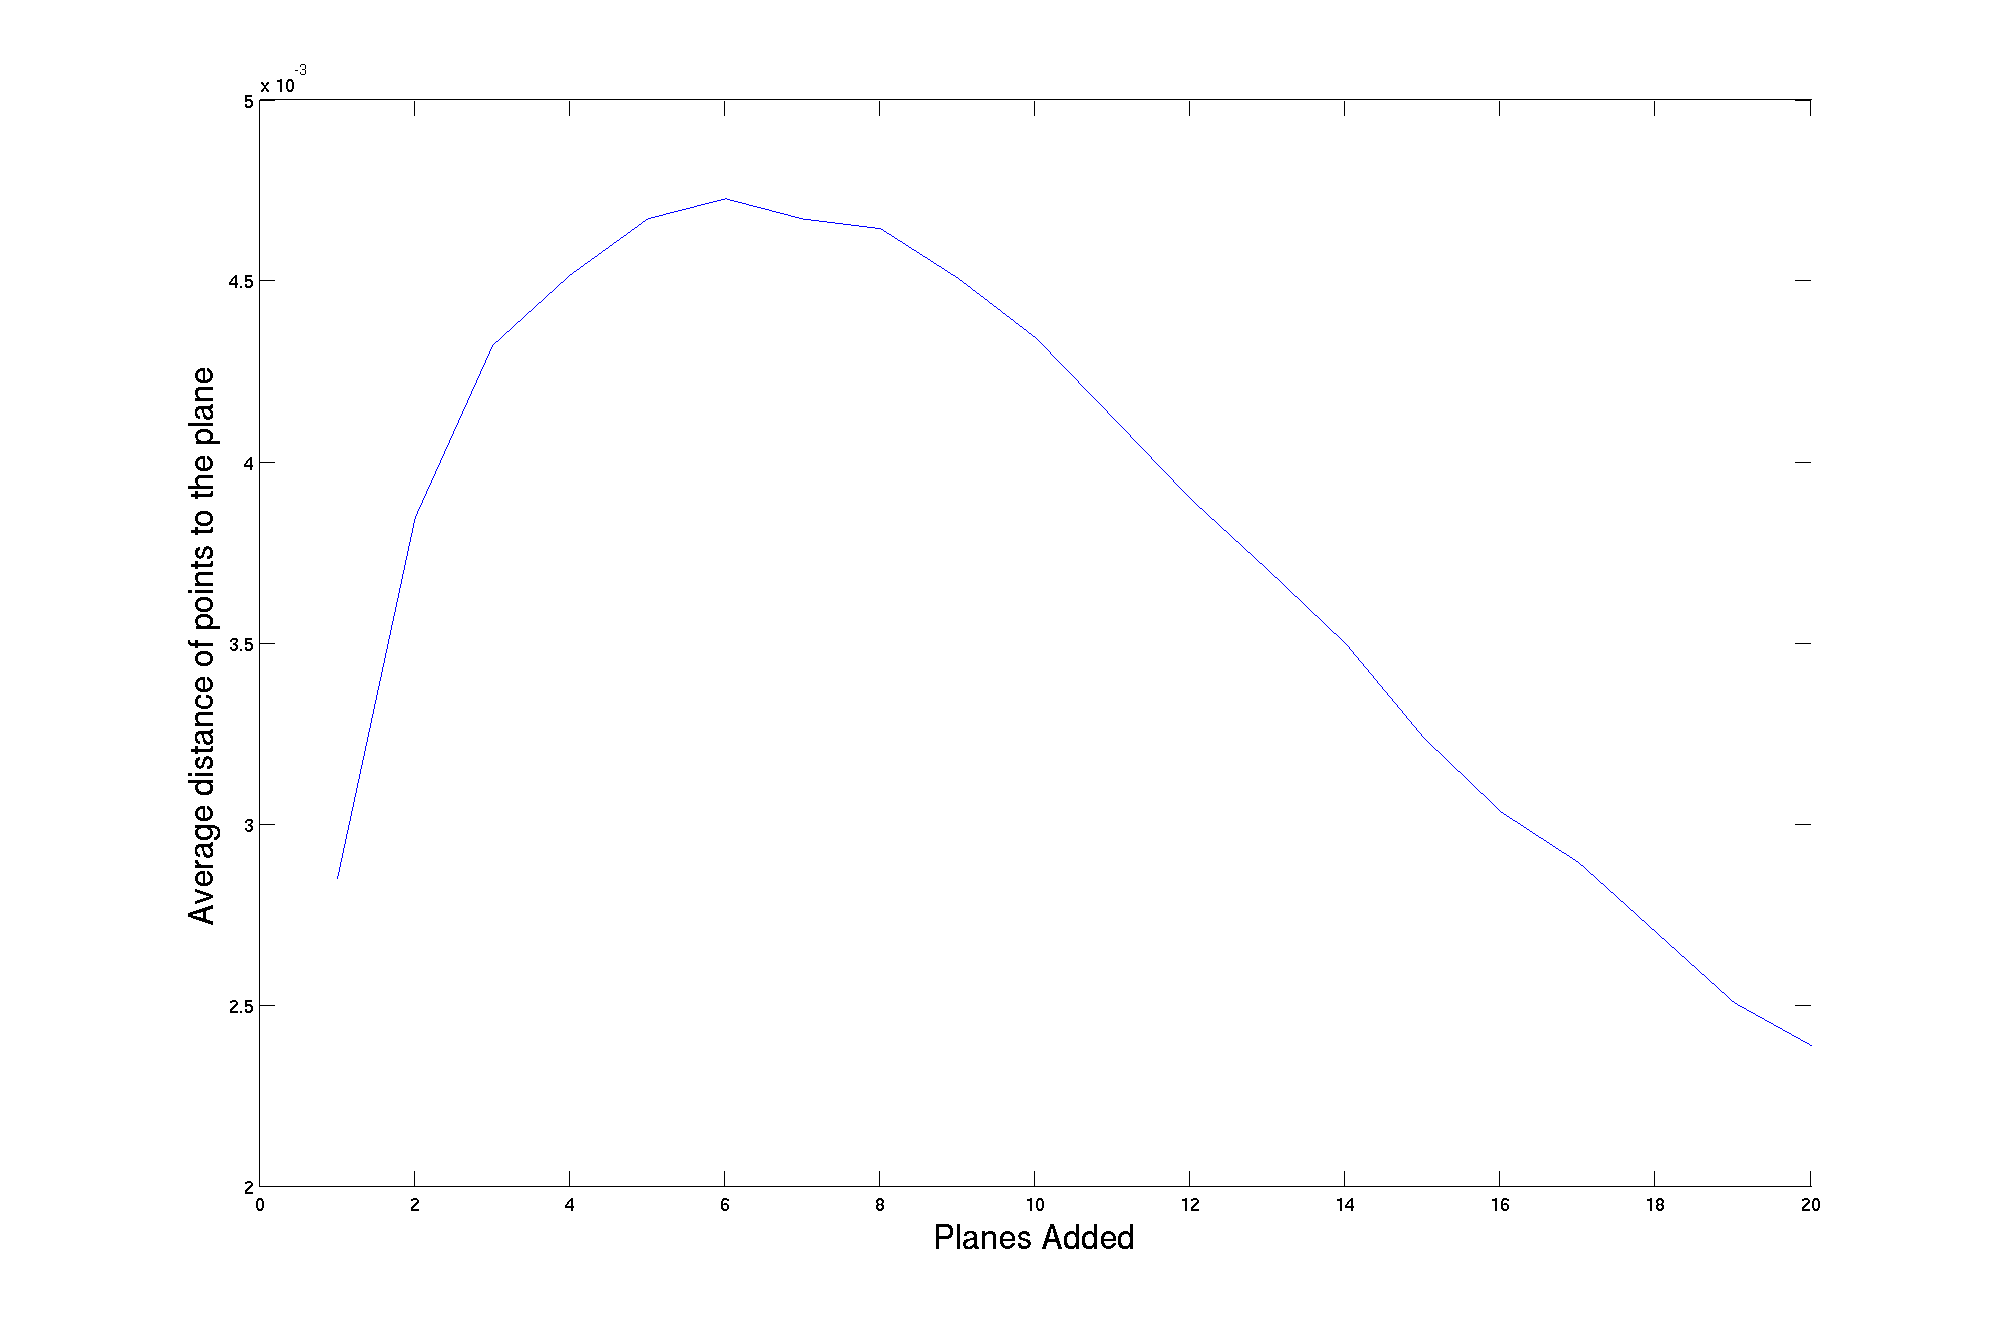
\includegraphics[width=1\textwidth]{figs/plane_angle_error_versus_foundation_plane}
  \caption{Absolute mean distance of every point in "S." region to the plane as a function of the number of frames in the composite data set.}
  \label{fig:plane_angle_error_versus_foundation_plane}
\end{figure}

\begin{thebibliography}{9}
  
\bibitem{lecture_code}
  ADVANCED VISION - TASK 4 MATLAB CODE
  \url{http://www.inf.ed.ac.uk/teaching/courses/av/MATLAB/TASK4/} 
  
\end{thebibliography}

\appendix

\section{Evaluation Figures}
On the following pages are all required figures from the evaluation section.

\begin{figure}[h!]
\centering
\subfigure[Frame 0]{
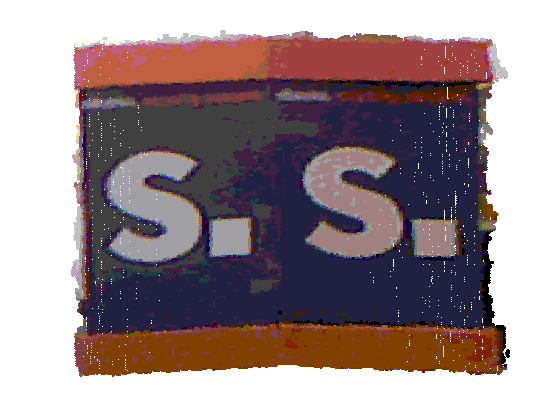
\includegraphics[width=0.30\linewidth]{../refactored/figures/part1_color_0_side}
}
\subfigure[Frame 1]{
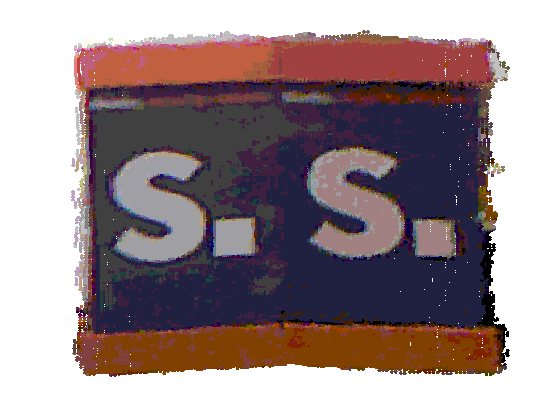
\includegraphics[width=0.30\linewidth]{../refactored/figures/part1_color_1_side}
}
\subfigure[Frame 2]{
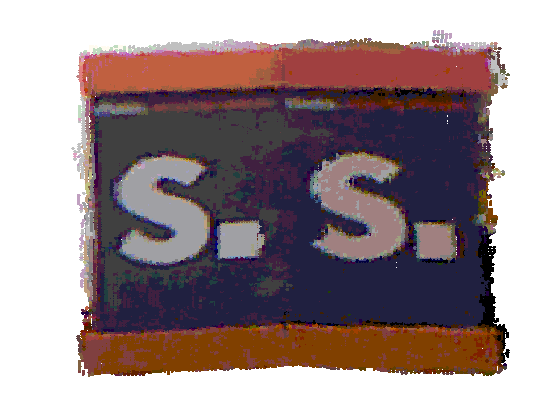
\includegraphics[width=0.30\linewidth]{../refactored/figures/part1_color_2_side}
}
\subfigure[Frame 3]{
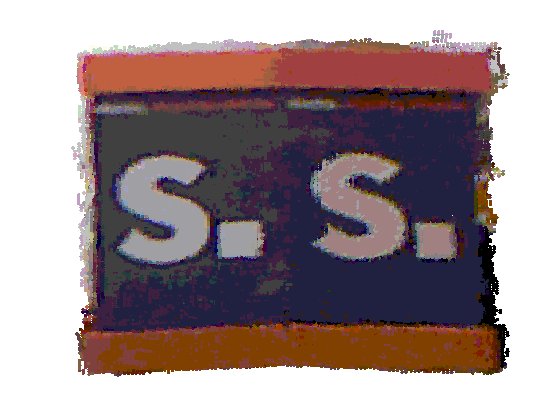
\includegraphics[width=0.30\linewidth]{../refactored/figures/part1_color_3_side}
}
\subfigure[Frame 4]{
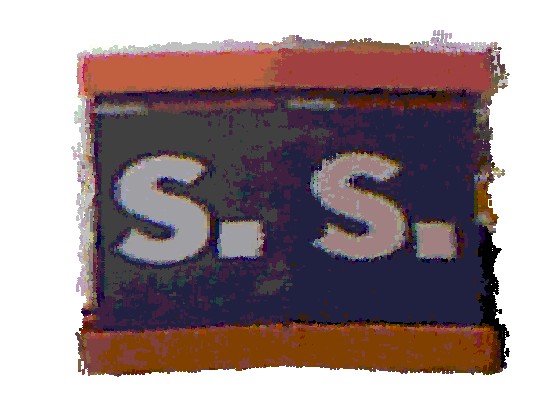
\includegraphics[width=0.30\linewidth]{../refactored/figures/part1_color_4_side}
}
\subfigure[Frame 5]{
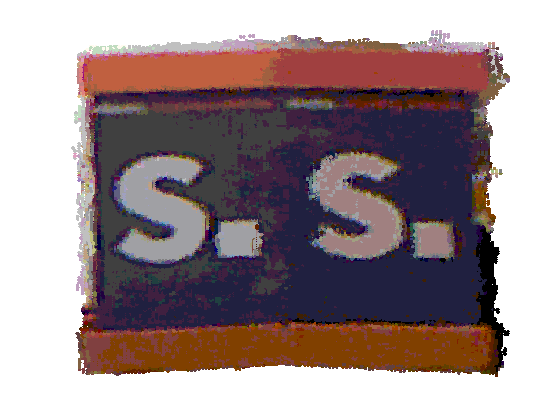
\includegraphics[width=0.30\linewidth]{../refactored/figures/part1_color_5_side}
}
\subfigure[Frame 6]{
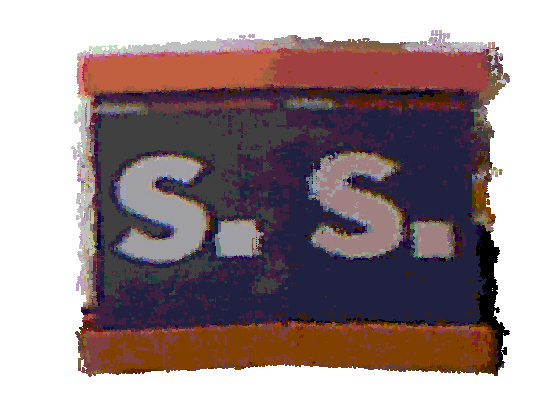
\includegraphics[width=0.30\linewidth]{../refactored/figures/part1_color_6_side}
}
\subfigure[Frame 7]{
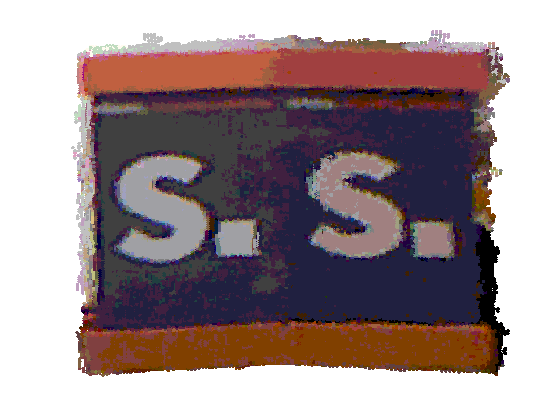
\includegraphics[width=0.30\linewidth]{../refactored/figures/part1_color_7_side}
}
\subfigure[Frame 8]{
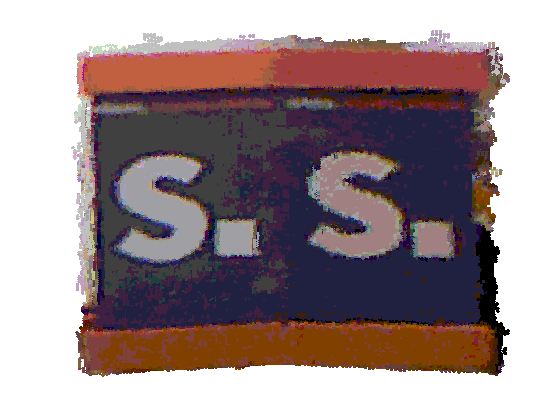
\includegraphics[width=0.30\linewidth]{../refactored/figures/part1_color_8_side}
}
\subfigure[Frame 9]{
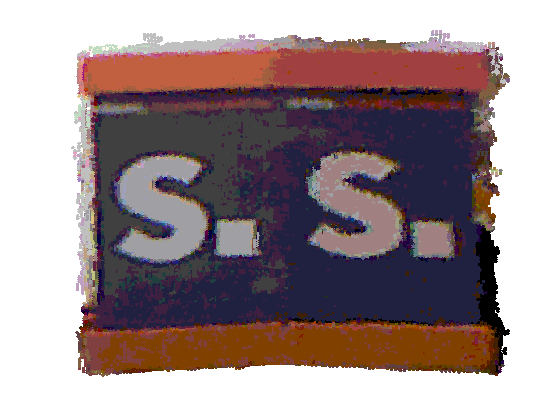
\includegraphics[width=0.30\linewidth]{../refactored/figures/part1_color_9_side}
}
\subfigure[Frame 11]{
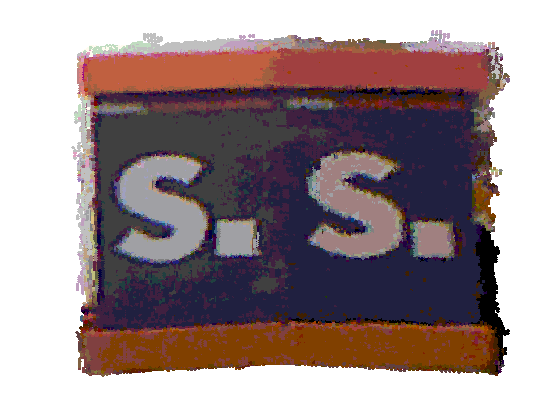
\includegraphics[width=0.30\linewidth]{../refactored/figures/part1_color_11_side}
}
\subfigure[Frame 12]{

\includegraphics[width=0.30\linewidth]{../refactored/figures/part1_color_12_side}
}
\subfigure[Frame 13]{

\includegraphics[width=0.30\linewidth]{../refactored/figures/part1_color_13_side}
}
\subfigure[Frame 14]{
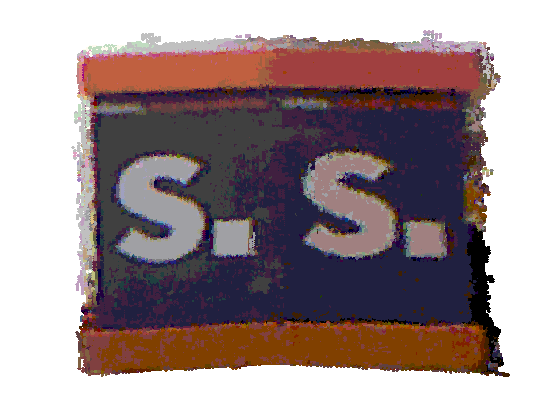
\includegraphics[width=0.30\linewidth]{../refactored/figures/part1_color_14_side}
}
\subfigure[Frame 15]{
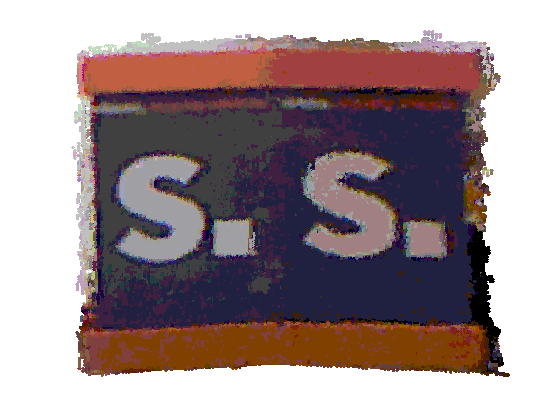
\includegraphics[width=0.30\linewidth]{../refactored/figures/part1_color_15_side}
}
\subfigure[Frame 16]{
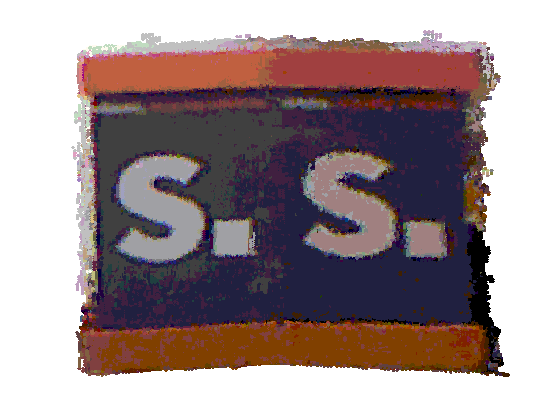
\includegraphics[width=0.30\linewidth]{../refactored/figures/part1_color_16_side}
}
\subfigure[Frame 17]{
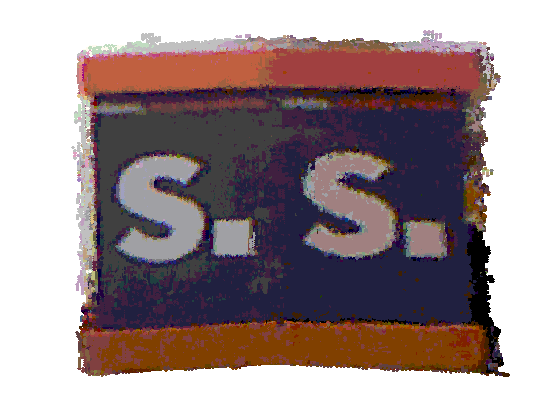
\includegraphics[width=0.30\linewidth]{../refactored/figures/part1_color_17_side}
}
\subfigure[Frame 18]{
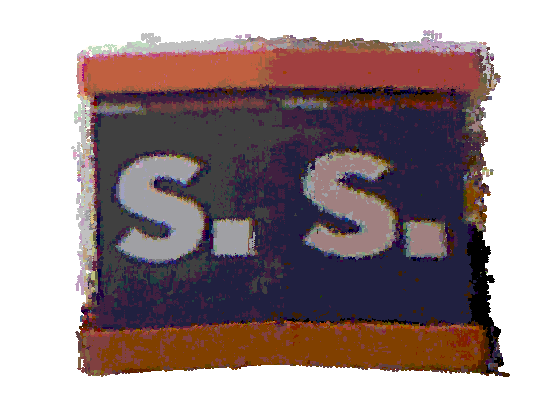
\includegraphics[width=0.30\linewidth]{../refactored/figures/part1_color_18_side}
}
\caption{Extracted boxes - side}
\label{fig:eval1a}
\end{figure}

\begin{figure}[h!]
\centering
\subfigure[Frame 19]{
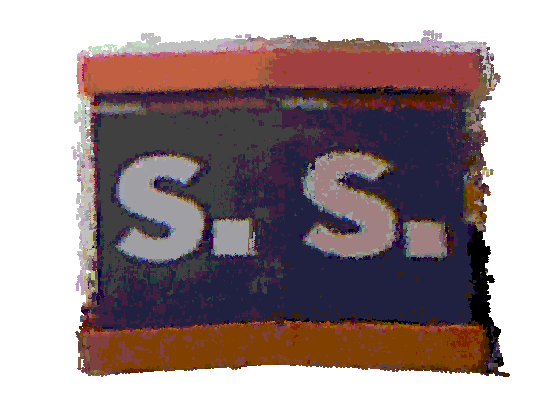
\includegraphics[width=0.30\linewidth]{../refactored/figures/part1_color_19_side}
}
\subfigure[Frame 20]{
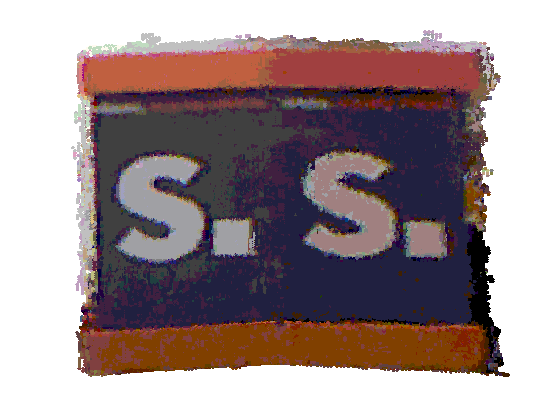
\includegraphics[width=0.30\linewidth]{../refactored/figures/part1_color_20_side}
}
\caption{Extracted boxes - side}
\end{figure}



\begin{figure}[h!]
\centering
\subfigure[Frame 0]{
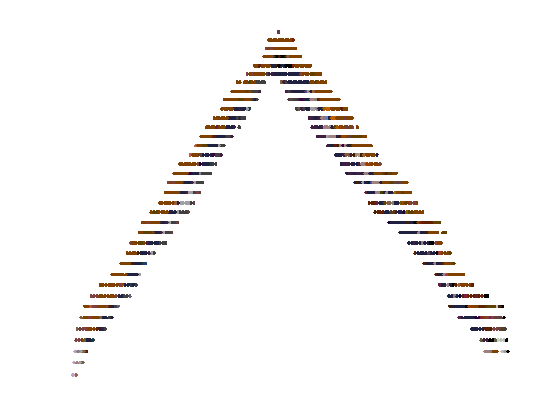
\includegraphics[width=0.30\linewidth]{../refactored/figures/part1_color_0_top}
}
\subfigure[Frame 1]{
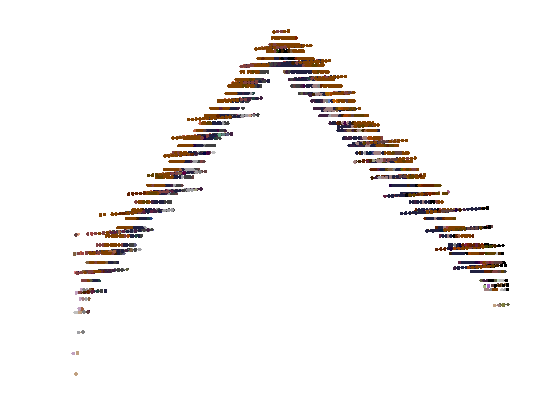
\includegraphics[width=0.30\linewidth]{../refactored/figures/part1_color_1_top}
}
\subfigure[Frame 2]{
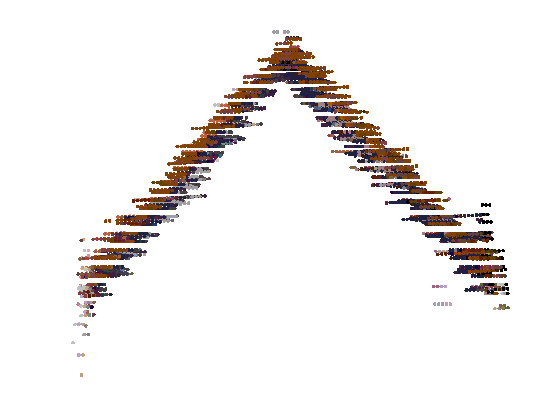
\includegraphics[width=0.30\linewidth]{../refactored/figures/part1_color_2_top}
}
\subfigure[Frame 3]{
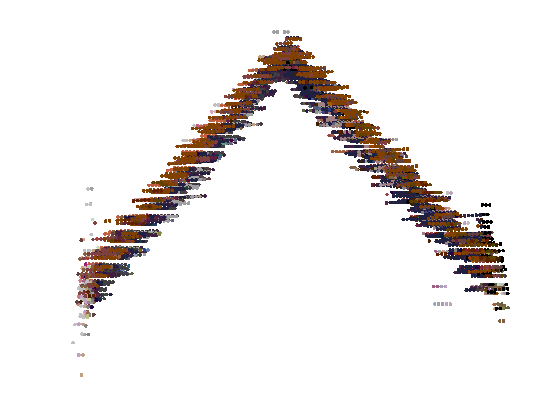
\includegraphics[width=0.30\linewidth]{../refactored/figures/part1_color_3_top}
}
\subfigure[Frame 4]{
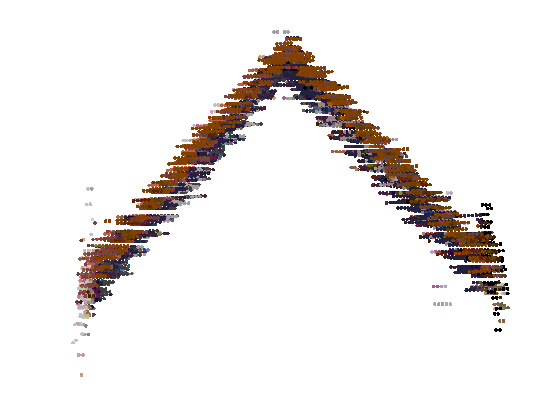
\includegraphics[width=0.30\linewidth]{../refactored/figures/part1_color_4_top}
}
\subfigure[Frame 5]{
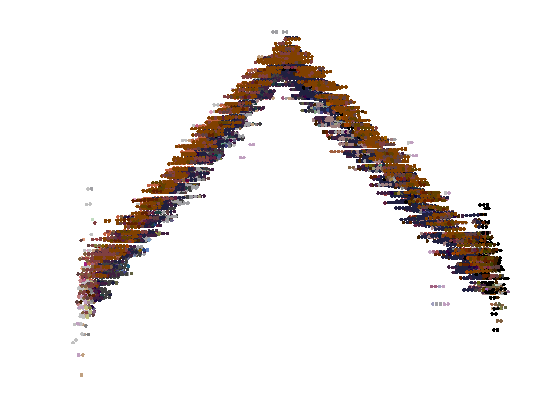
\includegraphics[width=0.30\linewidth]{../refactored/figures/part1_color_5_top}
}
\subfigure[Frame 6]{
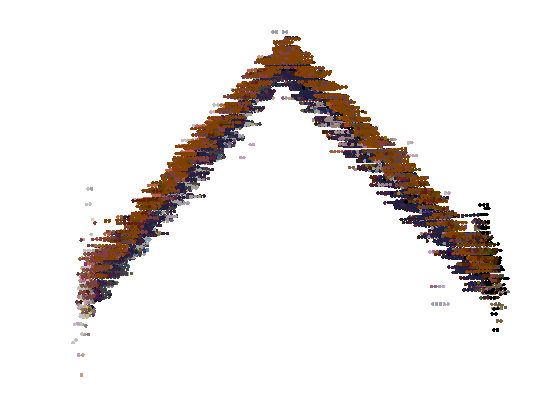
\includegraphics[width=0.30\linewidth]{../refactored/figures/part1_color_6_top}
}
\subfigure[Frame 7]{
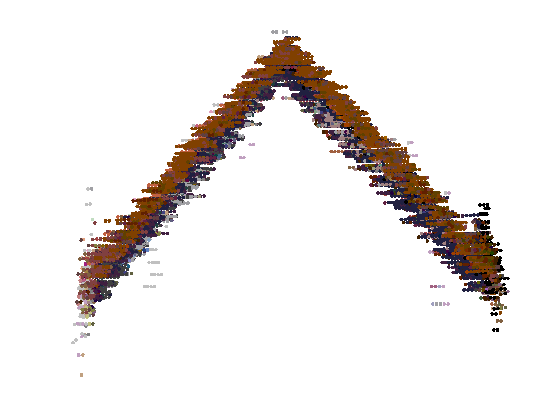
\includegraphics[width=0.30\linewidth]{../refactored/figures/part1_color_7_top}
}
\subfigure[Frame 8]{
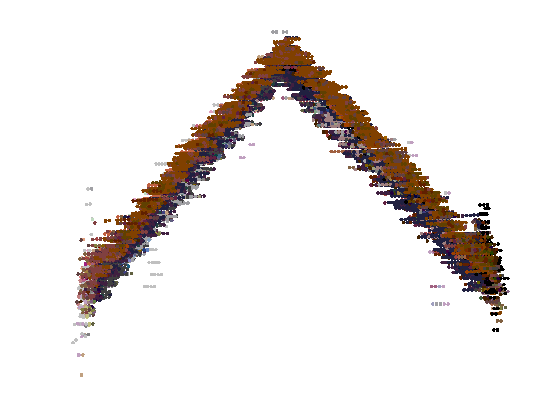
\includegraphics[width=0.30\linewidth]{../refactored/figures/part1_color_8_top}
}
\subfigure[Frame 9]{
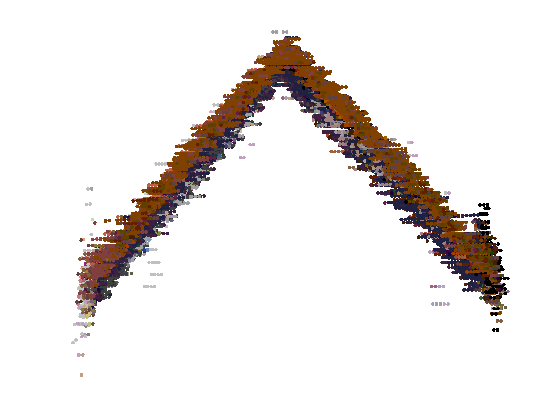
\includegraphics[width=0.30\linewidth]{../refactored/figures/part1_color_9_top}
}
\subfigure[Frame 11]{
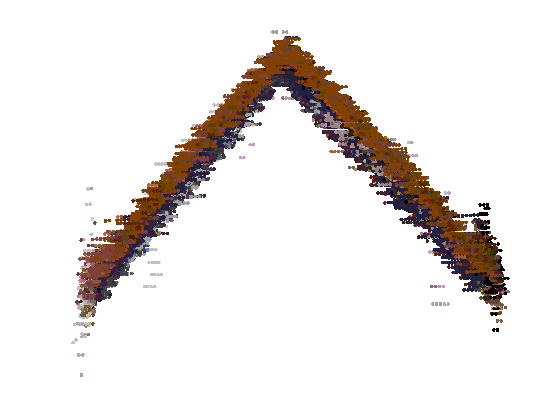
\includegraphics[width=0.30\linewidth]{../refactored/figures/part1_color_11_top}
}
\subfigure[Frame 12]{
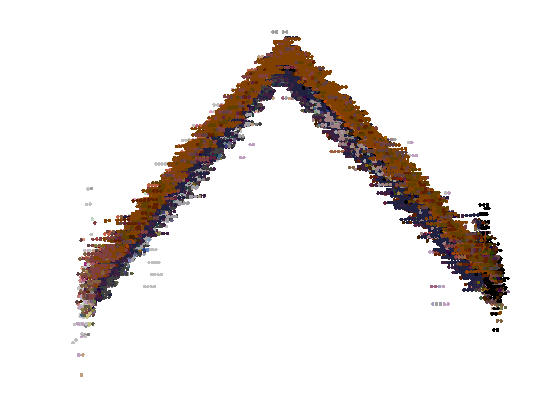
\includegraphics[width=0.30\linewidth]{../refactored/figures/part1_color_12_top}
}
\subfigure[Frame 13]{
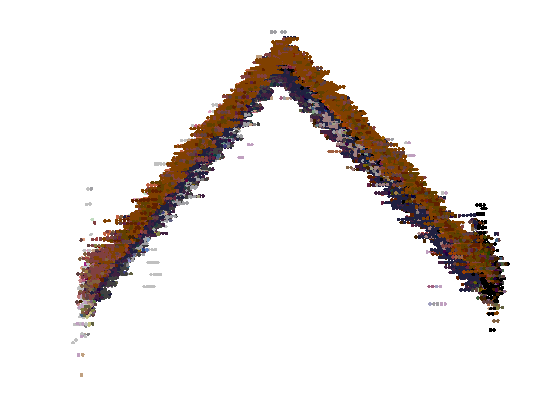
\includegraphics[width=0.30\linewidth]{../refactored/figures/part1_color_13_top}
}
\subfigure[Frame 14]{
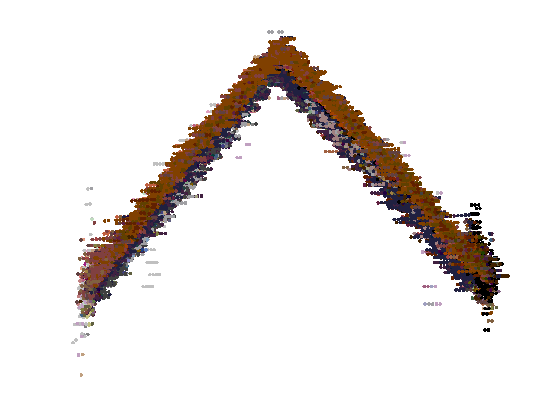
\includegraphics[width=0.30\linewidth]{../refactored/figures/part1_color_14_top}
}
\subfigure[Frame 15]{
\includegraphics[width=0.30\linewidth]{../refactored/figures/part1_color_15_top}
}
\subfigure[Frame 16]{
\includegraphics[width=0.30\linewidth]{../refactored/figures/part1_color_16_top}
}
\subfigure[Frame 17]{
\includegraphics[width=0.30\linewidth]{../refactored/figures/part1_color_17_top}
}
\subfigure[Frame 18]{
\includegraphics[width=0.30\linewidth]{../refactored/figures/part1_color_18_top}
}
\caption{Extracted boxes - top}
\end{figure}

\begin{figure}[h!]
\centering
\subfigure[Frame 19]{
\includegraphics[width=0.30\linewidth]{../refactored/figures/part1_color_19_top}
}
\subfigure[Frame 20]{
\includegraphics[width=0.30\linewidth]{../refactored/figures/part1_color_20_top}
}
\caption{Extracted boxes - top}
\end{figure}



\begin{figure}[h!]
\centering
\subfigure[Frame 0]{
\includegraphics[width=0.30\linewidth]{../refactored/figures/part1_range_0_side}}
\subfigure[Frame 1]{
\includegraphics[width=0.30\linewidth]{../refactored/figures/part1_range_1_side}}
\subfigure[Frame 2]{
\includegraphics[width=0.30\linewidth]{../refactored/figures/part1_range_2_side}}
\subfigure[Frame 3]{
\includegraphics[width=0.30\linewidth]{../refactored/figures/part1_range_3_side}}
\subfigure[Frame 4]{
\includegraphics[width=0.30\linewidth]{../refactored/figures/part1_range_4_side}}
\subfigure[Frame 5]{
\includegraphics[width=0.30\linewidth]{../refactored/figures/part1_range_5_side}}
\subfigure[Frame 6]{
\includegraphics[width=0.30\linewidth]{../refactored/figures/part1_range_6_side}}
\subfigure[Frame 7]{
\includegraphics[width=0.30\linewidth]{../refactored/figures/part1_range_7_side}}
\subfigure[Frame 8]{
\includegraphics[width=0.30\linewidth]{../refactored/figures/part1_range_8_side}}
\subfigure[Frame 9]{
\includegraphics[width=0.30\linewidth]{../refactored/figures/part1_range_9_side}}
\subfigure[Frame 11]{
\includegraphics[width=0.30\linewidth]{../refactored/figures/part1_range_11_side}}
\subfigure[Frame 12]{
\includegraphics[width=0.30\linewidth]{../refactored/figures/part1_range_12_side}}
\subfigure[Frame 13]{
\includegraphics[width=0.30\linewidth]{../refactored/figures/part1_range_13_side}}
\subfigure[Frame 14]{
\includegraphics[width=0.30\linewidth]{../refactored/figures/part1_range_14_side}}
\subfigure[Frame 15]{
\includegraphics[width=0.30\linewidth]{../refactored/figures/part1_range_15_side}}
\subfigure[Frame 16]{
\includegraphics[width=0.30\linewidth]{../refactored/figures/part1_range_16_side}}
\subfigure[Frame 17]{
\includegraphics[width=0.30\linewidth]{../refactored/figures/part1_range_17_side}}
\subfigure[Frame 18]{
\includegraphics[width=0.30\linewidth]{../refactored/figures/part1_range_18_side}}
\caption{Extracted depth points - side}
\end{figure}

\begin{figure}[h!]
\centering
\subfigure[Frame 19]{
\includegraphics[width=0.30\linewidth]{../refactored/figures/part1_range_19_side}}
\subfigure[Frame 20]{
\includegraphics[width=0.30\linewidth]{../refactored/figures/part1_range_20_side}}
\caption{Extracted depth points - side}
\end{figure}


\begin{figure}[h!]
\centering
\subfigure[Frame 0]{
\includegraphics[width=0.30\linewidth]{../refactored/figures/part1_range_0_top}}
\subfigure[Frame 1]{
\includegraphics[width=0.30\linewidth]{../refactored/figures/part1_range_1_top}}
\subfigure[Frame 2]{
\includegraphics[width=0.30\linewidth]{../refactored/figures/part1_range_2_top}}
\subfigure[Frame 3]{
\includegraphics[width=0.30\linewidth]{../refactored/figures/part1_range_3_top}}
\subfigure[Frame 4]{
\includegraphics[width=0.30\linewidth]{../refactored/figures/part1_range_4_top}}
\subfigure[Frame 5]{
\includegraphics[width=0.30\linewidth]{../refactored/figures/part1_range_5_top}}
\subfigure[Frame 6]{
\includegraphics[width=0.30\linewidth]{../refactored/figures/part1_range_6_top}}
\subfigure[Frame 7]{
\includegraphics[width=0.30\linewidth]{../refactored/figures/part1_range_7_top}}
\subfigure[Frame 8]{
\includegraphics[width=0.30\linewidth]{../refactored/figures/part1_range_8_top}}
\subfigure[Frame 9]{
\includegraphics[width=0.30\linewidth]{../refactored/figures/part1_range_9_top}}
\subfigure[Frame 11]{
\includegraphics[width=0.30\linewidth]{../refactored/figures/part1_range_11_top}}
\subfigure[Frame 12]{
\includegraphics[width=0.30\linewidth]{../refactored/figures/part1_range_12_top}}
\subfigure[Frame 13]{
\includegraphics[width=0.30\linewidth]{../refactored/figures/part1_range_13_top}}
\subfigure[Frame 14]{
\includegraphics[width=0.30\linewidth]{../refactored/figures/part1_range_14_top}}
\subfigure[Frame 15]{
\includegraphics[width=0.30\linewidth]{../refactored/figures/part1_range_15_top}}
\subfigure[Frame 16]{
\includegraphics[width=0.30\linewidth]{../refactored/figures/part1_range_16_top}}
\subfigure[Frame 17]{
\includegraphics[width=0.30\linewidth]{../refactored/figures/part1_range_17_top}}
\subfigure[Frame 18]{
\includegraphics[width=0.30\linewidth]{../refactored/figures/part1_range_18_top}}
\caption{Extracted depth points - top}
\end{figure}

\begin{figure}[h!]
\centering
\subfigure[Frame 19]{
\includegraphics[width=0.30\linewidth]{../refactored/figures/part1_range_19_top}}
\subfigure[Frame 20]{
\includegraphics[width=0.30\linewidth]{../refactored/figures/part1_range_20_top}}
\caption{Extracted depth points - top}
\label{fig:eval1b}
\end{figure}


\begin{figure}[h!]
\centering
\subfigure[Frame 0]{
\includegraphics[width=0.30\linewidth]{../refactored/figures/part2_0_left_square}}
\subfigure[Frame 1]{
\includegraphics[width=0.30\linewidth]{../refactored/figures/part2_1_left_square}}
\subfigure[Frame 2]{
\includegraphics[width=0.30\linewidth]{../refactored/figures/part2_2_left_square}}
\subfigure[Frame 3]{
\includegraphics[width=0.30\linewidth]{../refactored/figures/part2_3_left_square}}
\subfigure[Frame 4]{
\includegraphics[width=0.30\linewidth]{../refactored/figures/part2_4_left_square}}
\subfigure[Frame 5]{
\includegraphics[width=0.30\linewidth]{../refactored/figures/part2_5_left_square}}
\subfigure[Frame 6]{
\includegraphics[width=0.30\linewidth]{../refactored/figures/part2_6_left_square}}
\subfigure[Frame 7]{
\includegraphics[width=0.30\linewidth]{../refactored/figures/part2_7_left_square}}
\subfigure[Frame 8]{
\includegraphics[width=0.30\linewidth]{../refactored/figures/part2_8_left_square}}
\subfigure[Frame 9]{
\includegraphics[width=0.30\linewidth]{../refactored/figures/part2_9_left_square}}
\subfigure[Frame 11]{
\includegraphics[width=0.30\linewidth]{../refactored/figures/part2_11_left_square}}
\subfigure[Frame 12]{
\includegraphics[width=0.30\linewidth]{../refactored/figures/part2_12_left_square}}
\subfigure[Frame 13]{
\includegraphics[width=0.30\linewidth]{../refactored/figures/part2_13_left_square}}
\subfigure[Frame 14]{
\includegraphics[width=0.30\linewidth]{../refactored/figures/part2_14_left_square}}
\subfigure[Frame 15]{
\includegraphics[width=0.30\linewidth]{../refactored/figures/part2_15_left_square}}
\subfigure[Frame 16]{
\includegraphics[width=0.30\linewidth]{../refactored/figures/part2_16_left_square}}
\subfigure[Frame 17]{
\includegraphics[width=0.30\linewidth]{../refactored/figures/part2_17_left_square}}
\subfigure[Frame 18]{
\includegraphics[width=0.30\linewidth]{../refactored/figures/part2_18_left_square}}
\caption{Leftmost zoomed in square}
\label{fig:eval2a}
\end{figure}

\begin{figure}[h!]
\centering
\subfigure[Frame 19]{
\includegraphics[width=0.30\linewidth]{../refactored/figures/part2_19_left_square}}
\subfigure[Frame 20]{
\includegraphics[width=0.30\linewidth]{../refactored/figures/part2_20_left_square}}
\caption{Leftmost zoomed in square}
\label{fig:eval2b}
\end{figure}

\clearpage


\section{Code}
\label{apen:code_in}
\subsection{Main script}
\lstinputlisting[language=Matlab, caption=main\_script.m]
{"../refactored/main_script.m"}

\subsection{Box extraction}
\lstinputlisting[language=Matlab, caption=get\_box\_mask.m]
{"../refactored/Box extraction/get_box_mask.m"}

\subsection{Frame alignment}
\lstinputlisting[language=Matlab, caption=alignPointsToFoundationFrame.m]
{"../refactored/Frame alignment/alignPointsToFoundationFrame.m"}
\lstinputlisting[language=Matlab, caption=get\_box\_edges.m]
{"../refactored/Frame alignment/get_box_edges.m"}
\lstinputlisting[language=Matlab, caption=get\_point\_list.m]
{"../refactored/Frame alignment/get_point_list.m"}
\lstinputlisting[language=Matlab, caption=process\_foundation\_frame.m]
{"../refactored/Frame alignment/process_foundation_frame.m"}

\subsection{Plane fitting}
\lstinputlisting[language=Matlab, caption=plane\_kmeans.m]
{"../refactored/Plane fitting/plane_kmeans.m"}
\lstinputlisting[language=Matlab, caption=fit\_planes\_on\_composite\_dataset.m]
{"../refactored/Plane fitting/fit_planes_on_composite_dataset.m"}

\subsection{Evaluation}
\lstinputlisting[language=Matlab, caption=fit\_plane\_to\_s\_box.m]
{"../refactored/Evaluation/fit_plane_to_s_box.m"}





\end{document}
